\documentclass[conference]{IEEEtran}
\IEEEoverridecommandlockouts
% The preceding line is only needed to identify funding in the first footnote. If that is unneeded, please comment it out.

\usepackage{cite}
\usepackage{amsmath,amssymb,amsfonts}
\usepackage{algorithmic}
\usepackage{graphicx}
\usepackage{float}
\graphicspath{figures}

\usepackage{textcomp}
\usepackage{enumitem}
\usepackage{xcolor}
\def\BibTeX{{\rm B\kern-.05em{\sc i\kern-.025em b}\kern-.08em
    T\kern-.1667em\lower.7ex\hbox{E}\kern-.125emX}}
\begin{document}

\title{Concurrent Tree Traversals in Binary Search Trees\\
%{\footnotesize \textsuperscript{*}Note: Sub-titles are not captured in Xplore and
%should not be used}
\thanks{Identify applicable funding agency here. If none, delete this.}
}

\author{\IEEEauthorblockN{Robert Bland}
\IEEEauthorblockA{\textit{College of Engineering and Computer Science} \\
\textit{University of Central Florida}\\
Orlando, FL \\}
\and
\IEEEauthorblockN{Tyler Townsend}
\IEEEauthorblockA{\textit{College of Engineering and Computer Science} \\
\textit{University of Central Florida}\\
Orlando, FL \\}
}

\maketitle

\begin{abstract}
We introduce our reimplementation of what is considered a practical and concurrent binary search tree that maintains logical ordering information within the data structure, but our implementation will be transformed and compared against a transactional data structure. A transactional data structure will be implemented using software transactional memory which provides a system for executing atomic sections of code instead of using locks. This will allow for users to monitor memory locations that threads read and write to.
\end{abstract}

\begin{IEEEkeywords}
Search Trees, Concurrency, AVL, Data Structures
\end{IEEEkeywords}

\section{Introduction}
%Introduction should state the problem at hand and give some background %information and more about the progress and correctness. 
%Define and explain our topic as well the transactional data structure.
%Transactional data structure are

Concurrency is rampant in today's programming society and we are quickly adapting all serial data structures into concurrent data structures to actually benefit from our ever increasing core count of our CPU's. This now leads into our topic which covers two important and well known data structures, which are Binary Search Trees (BST) and Adelson-Velskii and Landis Trees (AVL). A Binary Search Tree is a node-based data structure that has a root that is the top of the tree and has two subtrees, which are the left and right subtree. The left subtree contains all nodes smaller than the current nodes key and the right subtree contains all nodes with keys greater than the current nodes key. An AVL Search tree is a modified BST, but now we also keep track of heights of all nodes, so that the left and right subtree height don't differ by more than one. If the differences between the two subtrees are greater than one then we rebalance the trees to keep the heights within that range to speed up our search time. The two trees must maintain two rules for our concurrent implementation, the first rule is that it cannot contain duplicates and the second rule is that it has to follow the standard BST/AVL structural layout.
	A potential problem is presented when implementing certain methods concurrently. Some questions that are brought up would be when to lock, the locking order and how can we implement a contains that is exceptionally fast and lightweight, since contains is typically called the most out of any method. Even with all this in mind the main question that hasn't been asked is now being answered, which is how do we generalize an implementation such that it can be applicable to any search tree and not just create specialized solutions [1]? The answer to such a practical search tree is one that introduces a condition for path traversal validation, such that it is applicable to any tree. The condition determines whether or not our key is in the tree by looking at the succinct path snapshot (SPS) and the traversal only needs to take a path limited by our succinct path snapshot. If the key is contained in one of the snapshots then the condition states that the key is in the tree otherwise it states that it does not exist in the tree.  Also, our snapshots will get modified if there are any changes or mutations to the tree or along a path. Using this idea of succinct path snapshots we can also extend it and create a lock-free implementation of contains since it now has a method to verify if our path has been modified without the need to traverse the tree again. This contains however, will traverse again if the verification method fails and because of this it cannot be wait-free since it could fail an indefinite amount of times (Sec 3).
	Our path condition also makes it possible to extend our implementation to allow for customized operations, such as rotations, without having to complicate our program any further. This will prove to be incredibly useful because one of our goals is to recreate our program to be a transactional data structure. A transactional data structure focuses on atomicity and on isolation to ensure that each action takes effect in sequential order.

%\section{Research}
%The research in this area, so compare to other papers?

\section{Implementation}
In this section we will be going over what each function does and describe the linearization points of each function (excluding TraverseNLock). We will also mention progress guarantee, correctness condition and synchronization techniques (NOTE: Maybe move this technique idea to design). The functions to be described are Contains(), Insert(), Remove(), UpdateSnaps() and TraverseNLock(). We will also describe how we initialize our tree and our sentinel nodes. Important note is that every node has an atomic mark designating whether or not it has been logically removed.
\subsection{Tree and Nodes}
Our tree implementation is very familiar if one has seen a standard BST tree, since items less than the current key go down the left path and items greater than the current node go on the right path, but one core idea that our tree follows is that we can only add nodes at the end of the tree and not in between two nodes. We can still remove nodes anywhere in the tree and in one scenario we will actually swap nodes, but for more information on that check the Remove() section. Our tree is initialized to have two sentinel nodes to handle edge cases and the first item we insert will become the root. Our nodes implementation for our concurrent method is different then what we had for our serialized implementation and it will look like this :
\begin{enumerate}
\item T Key
\item Atomic Snapshot (consists of two nodes)
\item Node* LeftChild
\item Node* RightChild
\item Node* Parent
\item Height (For AVL)
\end{enumerate}
We must also keep track of our parent so that we can traverse up the tree when doing certain methods and to help maintain our locking-order, discussed in design decisions.
\subsection{Snapshots}
Snapshots are an integral part of our design because it will guarantee that our contains will not miss any elements that have been moved since it has started. We implemented it by having each node contain a succinct snapshot that contains itself and its successor or predecessor[2(Power Point Slides One)]. This will create an implicit list of nodes with keys in ascending order, note that it isn't linked so we cannot traverse through that list with our contains. We do not search through this linked list, but if the item is not within that list then we can say that it does not exist.
\subsection{UpdateSnaps}
The UpdateSnaps() function called by Insert() or Remove() to update the succinct snapshots of every node that has been changed by the that Insert() or Remove() call. UpdateSnaps() takes one of the following as its parameters:
\begin{enumerate}[label=(\roman*)]
	\item A Node
	\item A Node plus condition
	\item Four Nodes
\end{enumerate}
(I) is used only for Inserts() since we only care about changing that, Remove() will call (II) if the left and right node are leaves or if the right node is its successor and (III) is called when the node being removed has two children and its right child has left child, which will be our nodes successor. This function is recursive and locks nodes if Remove() has called it to change the parents succinct. 
\subsection{Contains}
The Contains() function that we have developed has to be lock-free or there was no point in recreating this paper, so when we develop it we can only use compare-and-swaps. Knowing this we have developed it to at most only use one compare-and-swap, which will be used if we do not find the item. Our contains will have two scenarios happen, either the item has been found when we traverse from the root with our key or we have reached a leaf and cannot find the item.
Our implementation has a lock-free contains and a deadlock-free insert and removes. Our contains() is lock-free because it only uses compare-and-swap, which has a consensus number of infinity, so by only using that atomic operation in that function we can say that even if it fails at least one other operation managed to succeed. If we find our item/key at a node in the list then we check if has been logically removed with a marking on that node and if it not marked then we return true otherwise we restart. This trait proves that this implementation is not starvation-free so it is not wait-free as well. If Contains() could not find the item/key then it reads the succinct snapshot of the node and checks whether or not it is contained in that snapshot. If it is then that means the node has been swapped out and it will restart to find it otherwise we return false.
\subsection{TraverseNLock}
TraverseNLock() will lock the node we are trying to find or a leaf in the tree, if we didn't find our key. Our implementation is identical to Contains() except that it contains locks and returns our node that is now locked instead of a boolean. There are two possible places that we lock, the first being right after we check the marking of our item/key if we found it. The second possible place to lock our node is right before reading the succinct path snapshot to guarantee, which will guarantee that no contaminated data in the set if we do it here.
\subsection{Insert}
A concurrent insert is very similar to a sequential insert with the only difference being that we need to update our snapshots. Our insert first starts by taking in a key and uses TraverseNLock, which returns a node that we locked, to find out where our key belongs. If this node is our key then we unlock the node and return false since we do not allow for duplicates. If we didn't find our key then the node locked will be our parent and we will create a node that contains our key. We then set the parent point of the newly created node to our locked parent node. We then set our parent nodes left or right node pointer, depending on whether or not our key is less than or greater than our parents key, to our newly created node. Then we update the snapshots of our newly created node, unlock our parent node and finally returns true.
\subsection{Remove}
A concurrent remove will take in a key k to remove from our tree and if it returns false otherwise it returns true. First remove will find and lock the node containing our key using TraverseNLock. If we didn't find the node containing our key then we return false.Then it follows one of three scenarios
\begin{enumerate}
\item If the locked node has one child then we first mark the node as removed, which is the linearization point, then we update our snaps, unlock all the nodes it locked and returns true.
\item If the locked node has two children and our right child has no left child then first mark the locked node as removed. Then we set our parents right node to be our right child and our right child will point to our left child, then we update snaps, unlock all the nodes it locked and returns true.
\item If the locked node has two children and our right child has a left child, we first mark our node for removal. Then we have to traverse through the tree and attempt to lock our successor, which restarts when it fails. If we successfully lock our successor then we lock the successors parent to change its left pointer to the successors right child, if it has one. We then swap our successor and locked node, update snaps, unlock all the nodes it locked and returns true.
\end{enumerate}  
\section{Design Decisions}

%locking-order

%TALK ABOUT HOW WE DIDN'T USE A LIST FOR SNAPSHOTS

%TALK ABOUT WHY WE LOCK BEFORE THE READ

%Locking Order as well

We designed our implementation to mirror the pseudo-code of the paper in [1]. This came with benefits of being able to efficiently program and recreate most of what the authors intended for us to implement. However, there were also some challenges as well since they intentionally left out where to include some locks in the pseudo-code and omitted some parts of the code for updating our snapshots. They did mention the potential location of each lock or where certain critical sections are with respect to the pseudo-code and presented some locations for putting locks in the insert and removal implementations. By leaving out some locations this give us enough leeway to interpret when we should use locks in our UpdateSnaps() function, but we have to implement to maintain correctness for our algorithm.
	One common problem when designing concurrent structures is addressing deadlocks and preventing such scenarios from happening. First we should expand on what a deadlock is. A deadlock occurs when one thread locks a resource and needs another resource that another thread has locked and that other thread also needs the first threads resource before unlocking its own resource. This creates a cyclic dependency and thus we can say that that algorithm is prone to deadlocking. We solve this problem by implementing a general locking order that all methods will follow. When traversing we will lock from the bottom-most leaf and work up the tree. When we break this ordering, by locking a node that isn't a leaf, we will attempt to lock nodes below us, so that if it fails we will release our lock. If we didn't release our lock on a failed attempt then we will create this cyclic dependency mentioned earlier and create a deadlock scenario which will ruin our correctness condition.
	Linearization is important when mentioning the correctness condition of our algorithm. So a linearization point is the point in time, usually a line of code, when a method/function operation can be seen by other threads. In the case of adding we say that the linearization point is when our node is reachable from our parent that we added ourselves to. A remove is linearized once we mark our node for removal. Contains has two linearization points however, the first linearization point of contains is with respect to a remove and its a race to see who can read or mark the node they are searching for. The second linearization point is when the node isn't found and we check the atomic snapshot. Since the snapshot can possibly be modified by a remove or add before we check that snapshot, so if we check that and we cannot find our key in that snapshot then we can say that the key isn't in the list and can return false.

\section{Testing}

Our testing is comprised of two parts for increased clarity. Our first part consists of the technical details of how we created our experiments and what we tested it on and compare the tests to. The second part focuses on what our results were and what it means.

\subsection{Set-Up For Experiments}
Before we begin testing we must first realize that we use C++ while they use Java, so ours should theoretically perform faster than the original implementation due to Java overhead. Our tests thread count will be smaller in our testing when compared to the original tests because our requirements for testing have to be smaller in scale, so it is possible for our reimplementation to not perform as well as the original for higher thread counts. With that in mind we evaluated our internal BST and internal AVL tree and compared them to other recent implementations and our transactional data structure. We compared our BST to the results given to us by [1 (The Paper)] as well as LO-BST, which is a lock-based internal BST, and the transactional data BST implementation. We then compared our internal AVL tree to the results given to us by [1 (The Paper)] and to LO-AVL, which is a lock-based internal AVL tree, and our transactional data AVL implementation. 
We ran these experiments on a [INSERT PROCESSOR, RAM, Cores, Processors with how many cores, and whether it allows for hyperthreading, OS that it ran on(Probably Linux) with version, What IDE and environment that we ran it on as well].
We try to keep consistency with the original implementation with our experiments, so we directly copied their experiments for accurate comparisons by following a “standard empirical evaluation” [1] (Put 7,8,12 from their paper since that is referenced) . Our experiments will be executing a series of five-second trials and will be comparing the number of operations each one executes within that time frame. The trials will be ran ten times for our two implementations and averaged out and compared to the results given in Table 1 (from paper [1]). There will be 3 different test scenarios for every implementation with each scenario having its own unique workload. The three scenarios are : 
\begin{enumerate}[label=(\roman*)]
	\item 90\% contains, 9\% insert, 1\% remove
	\item 70\% contains, 20\% insert, 10\% remove
	\item 0\% contains, 50\% inserts, 10\% removes
\end{enumerate}

\subsection{Results}

%Results go here and compare what we got to what they got
%Also put 9 graphs up for each distribution of operations and transaction size
\begin{figure}[H]
\begin{tabular}{c}
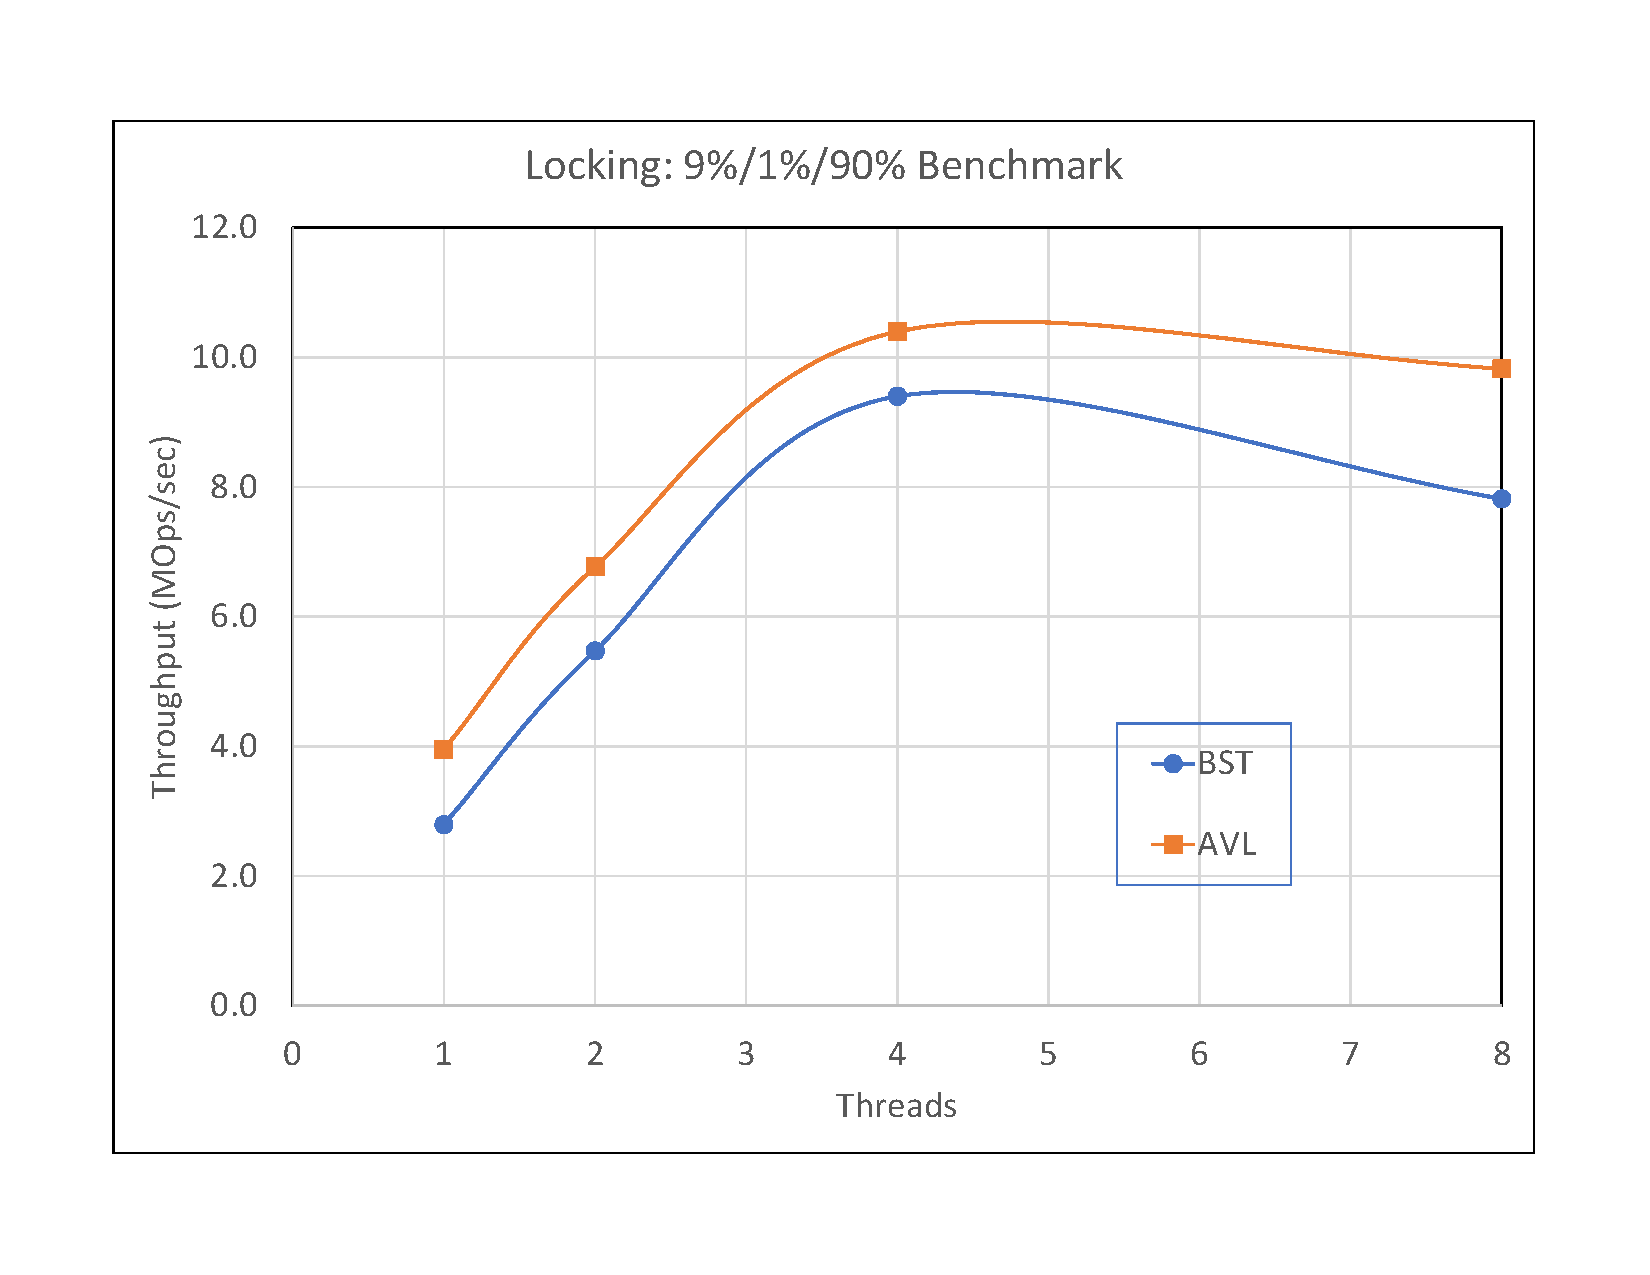
\includegraphics[width =\linewidth]{figures/conc-9-1-90}\\
(a) \\
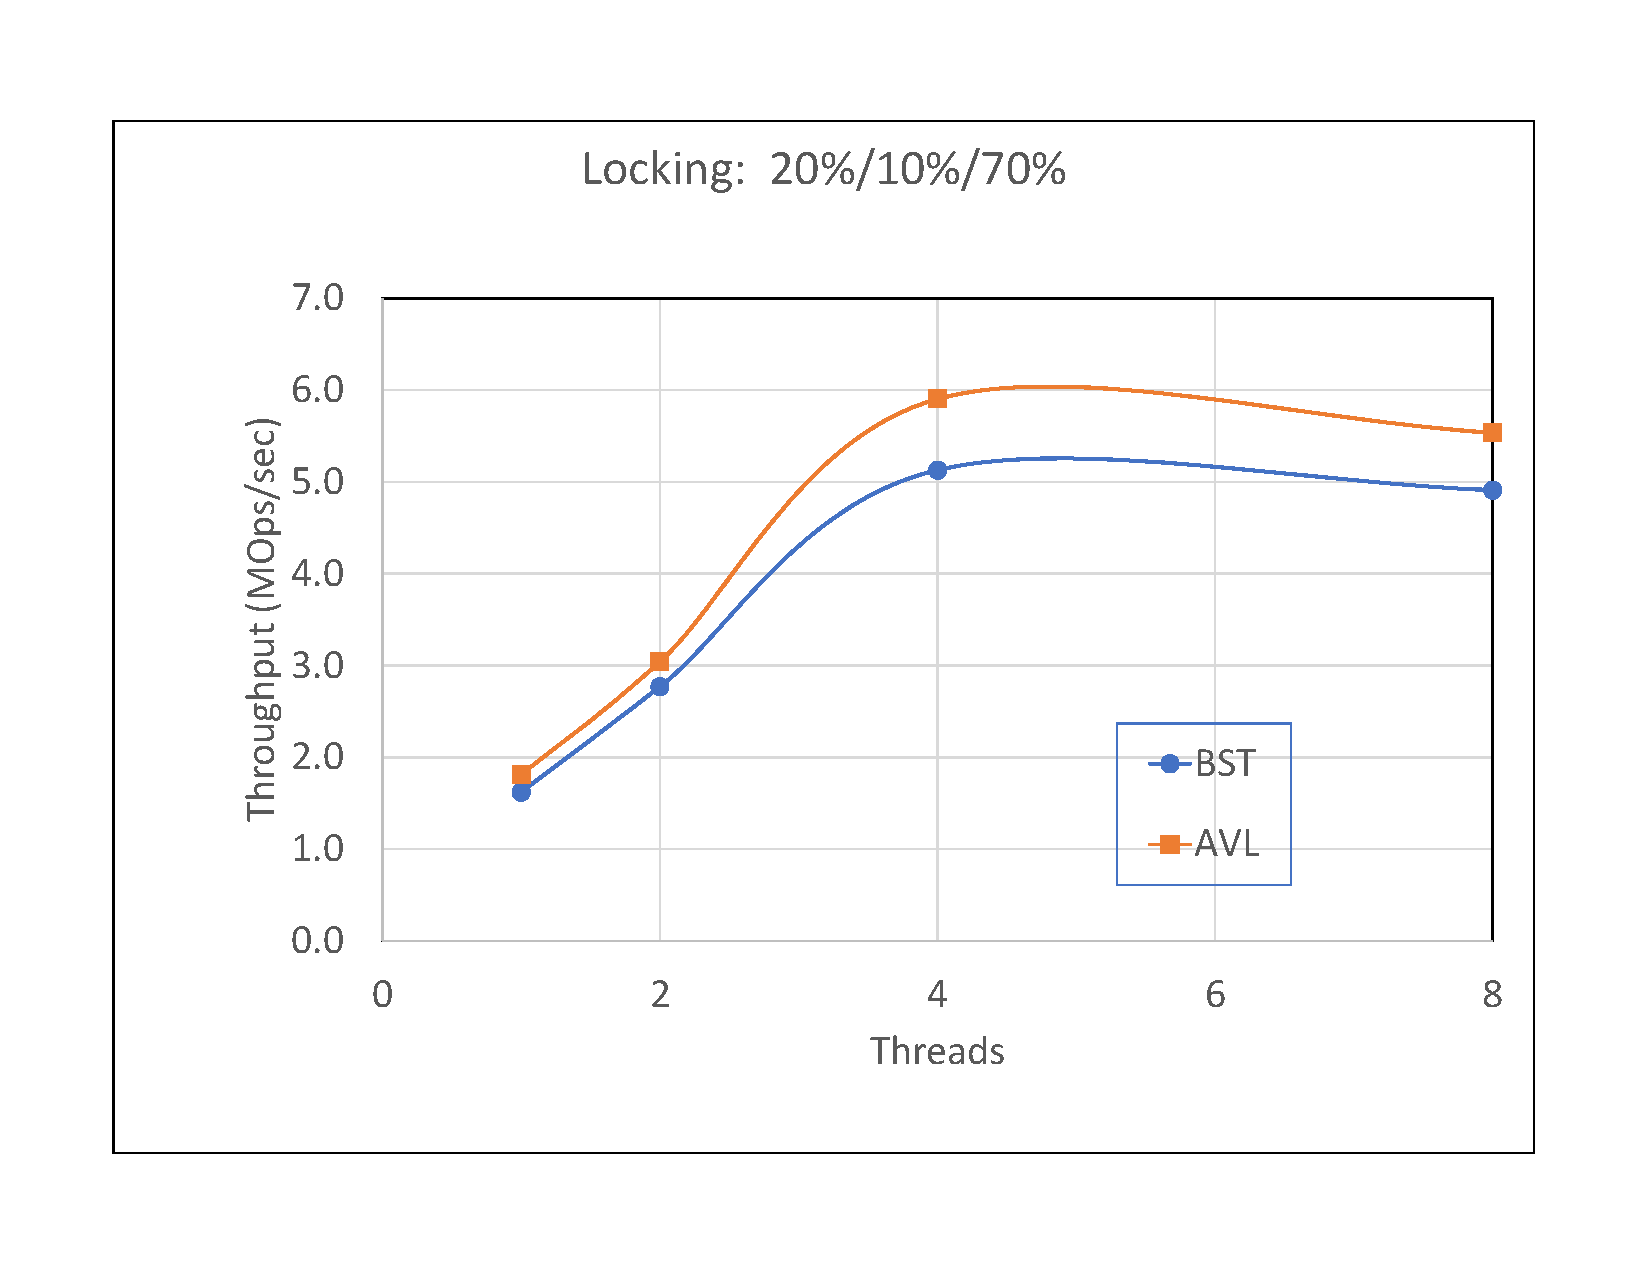
\includegraphics[width =\linewidth]{figures/conc-20-10-70}\\
(b) \\
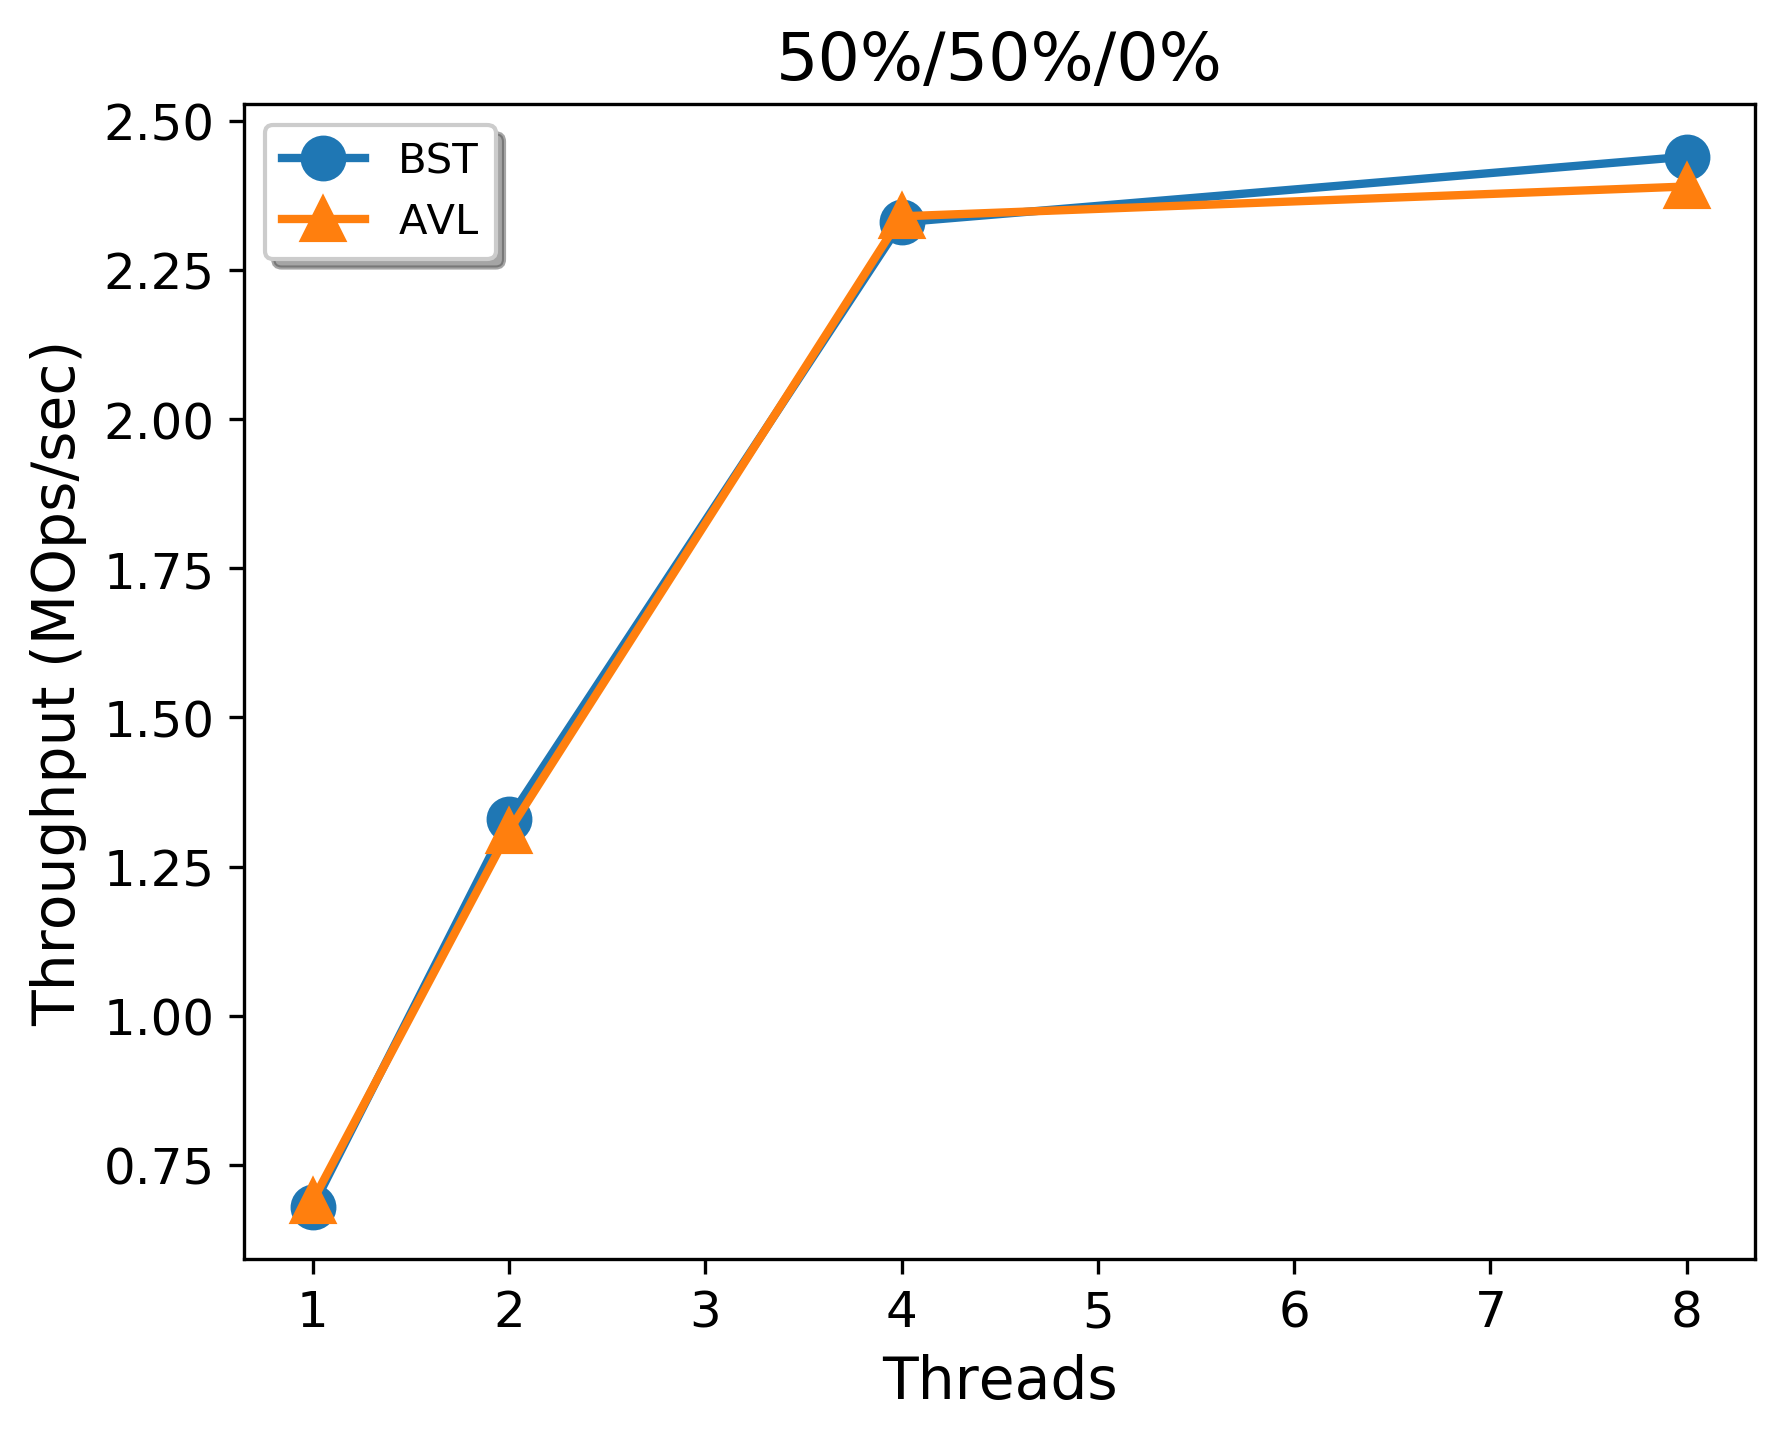
\includegraphics[width =\linewidth]{figures/conc-50-50-0} \\
(c) 
\end{tabular}
\caption{adsf}
\end{figure}

\begin{figure}[H]
\begin{tabular}{c}
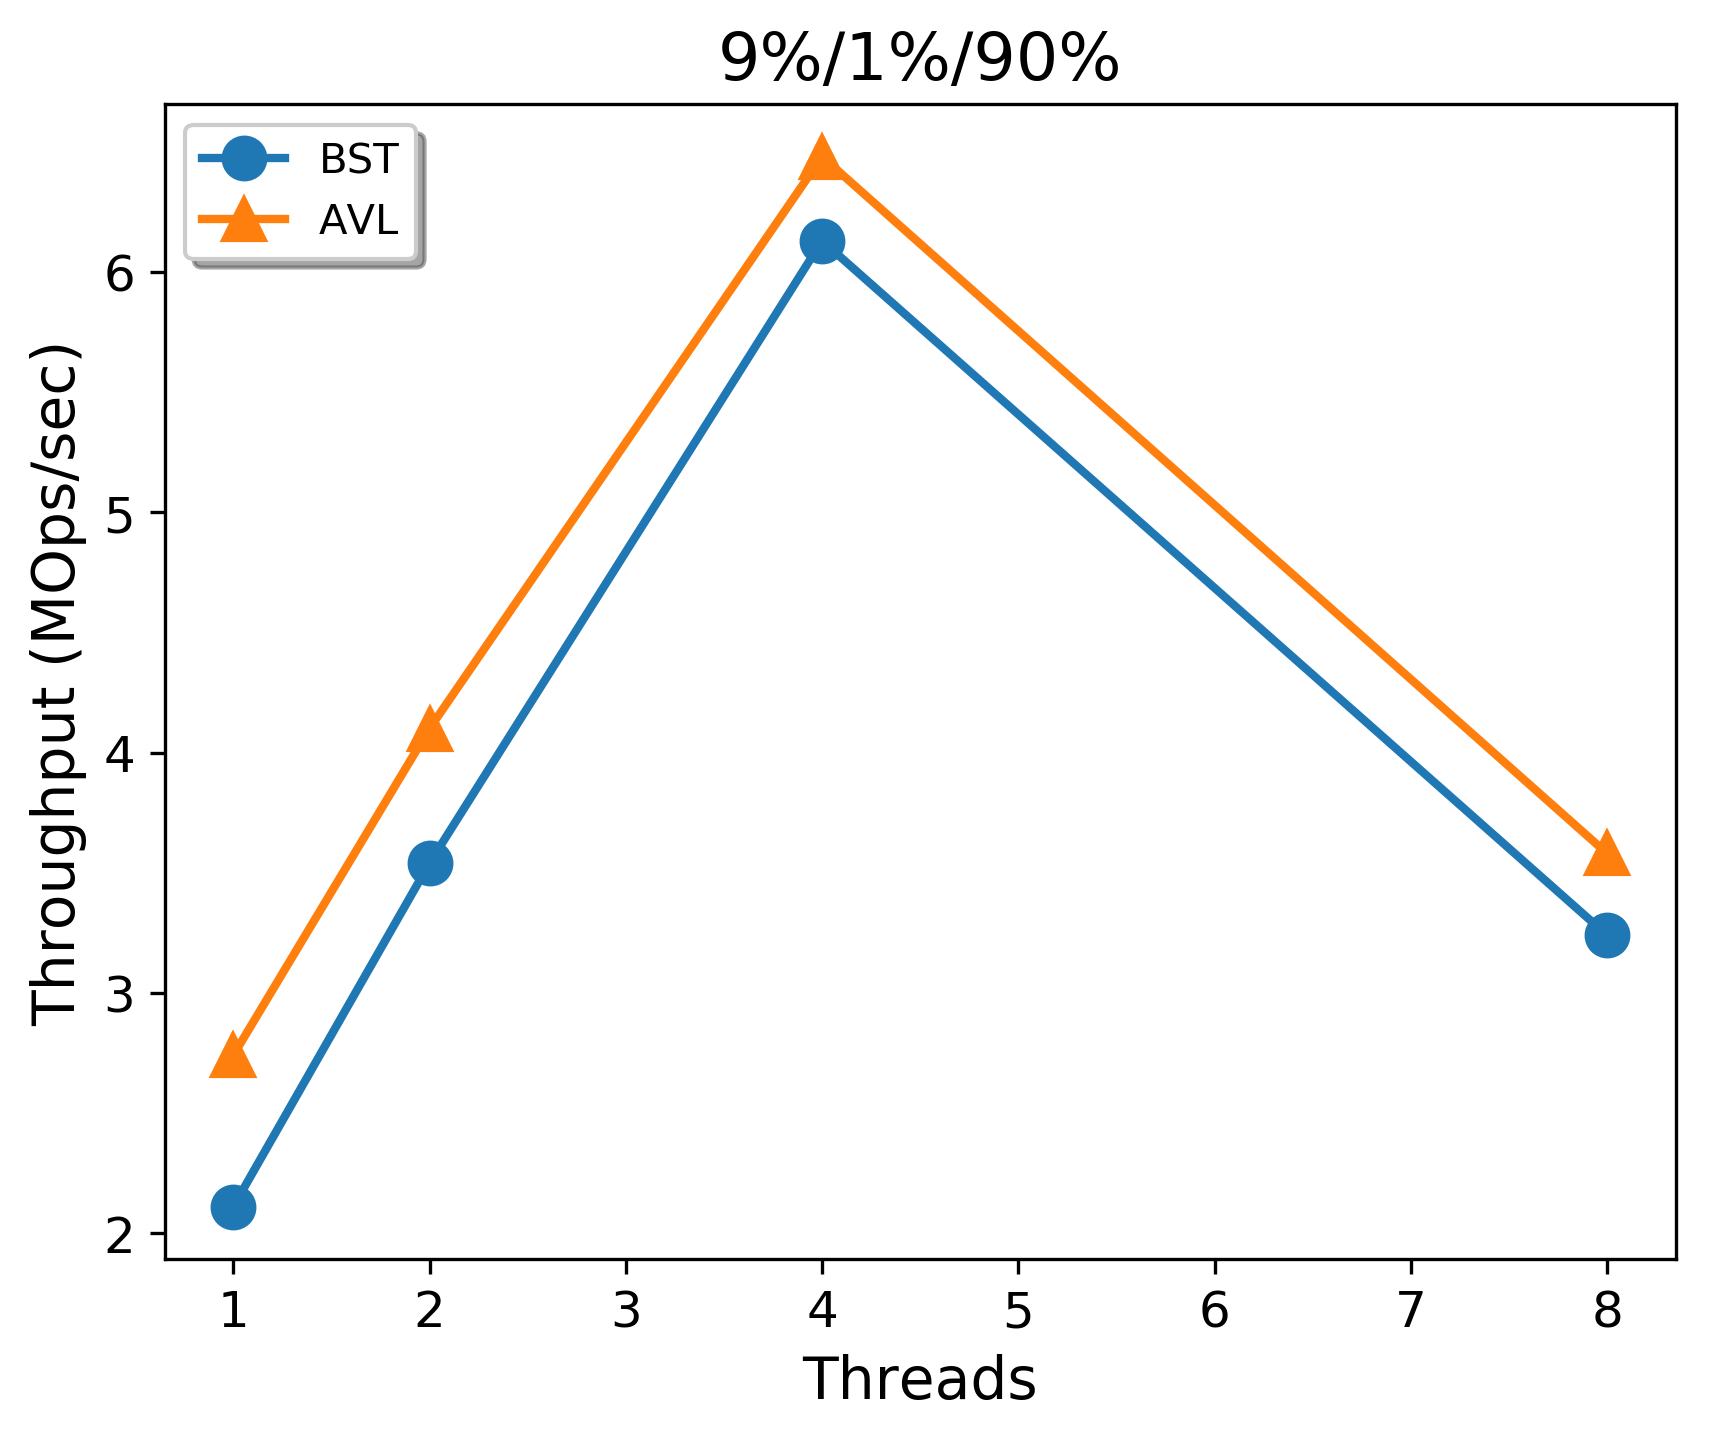
\includegraphics[width =\linewidth]{figures/stm1-9-1-90}\\
(a) \\
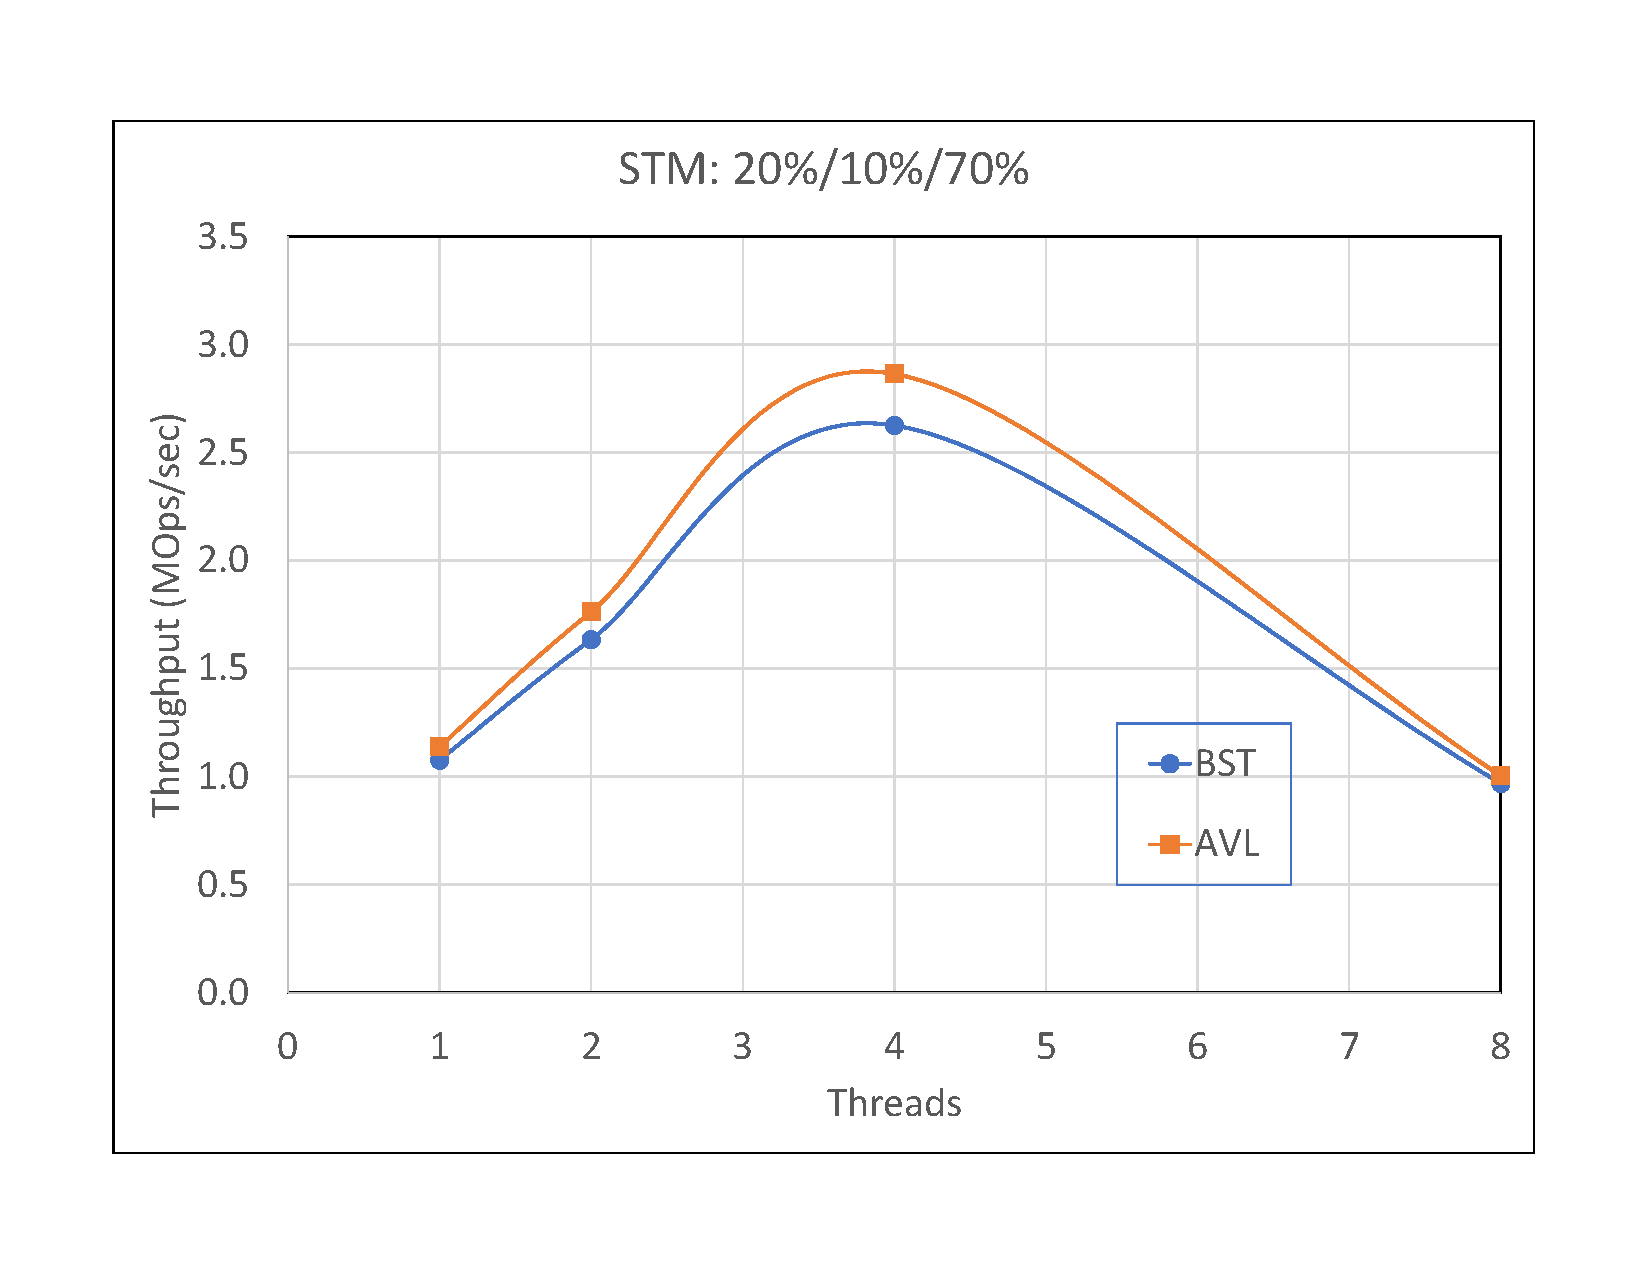
\includegraphics[width =\linewidth]{figures/stm1-20-10-70}\\
(b) \\
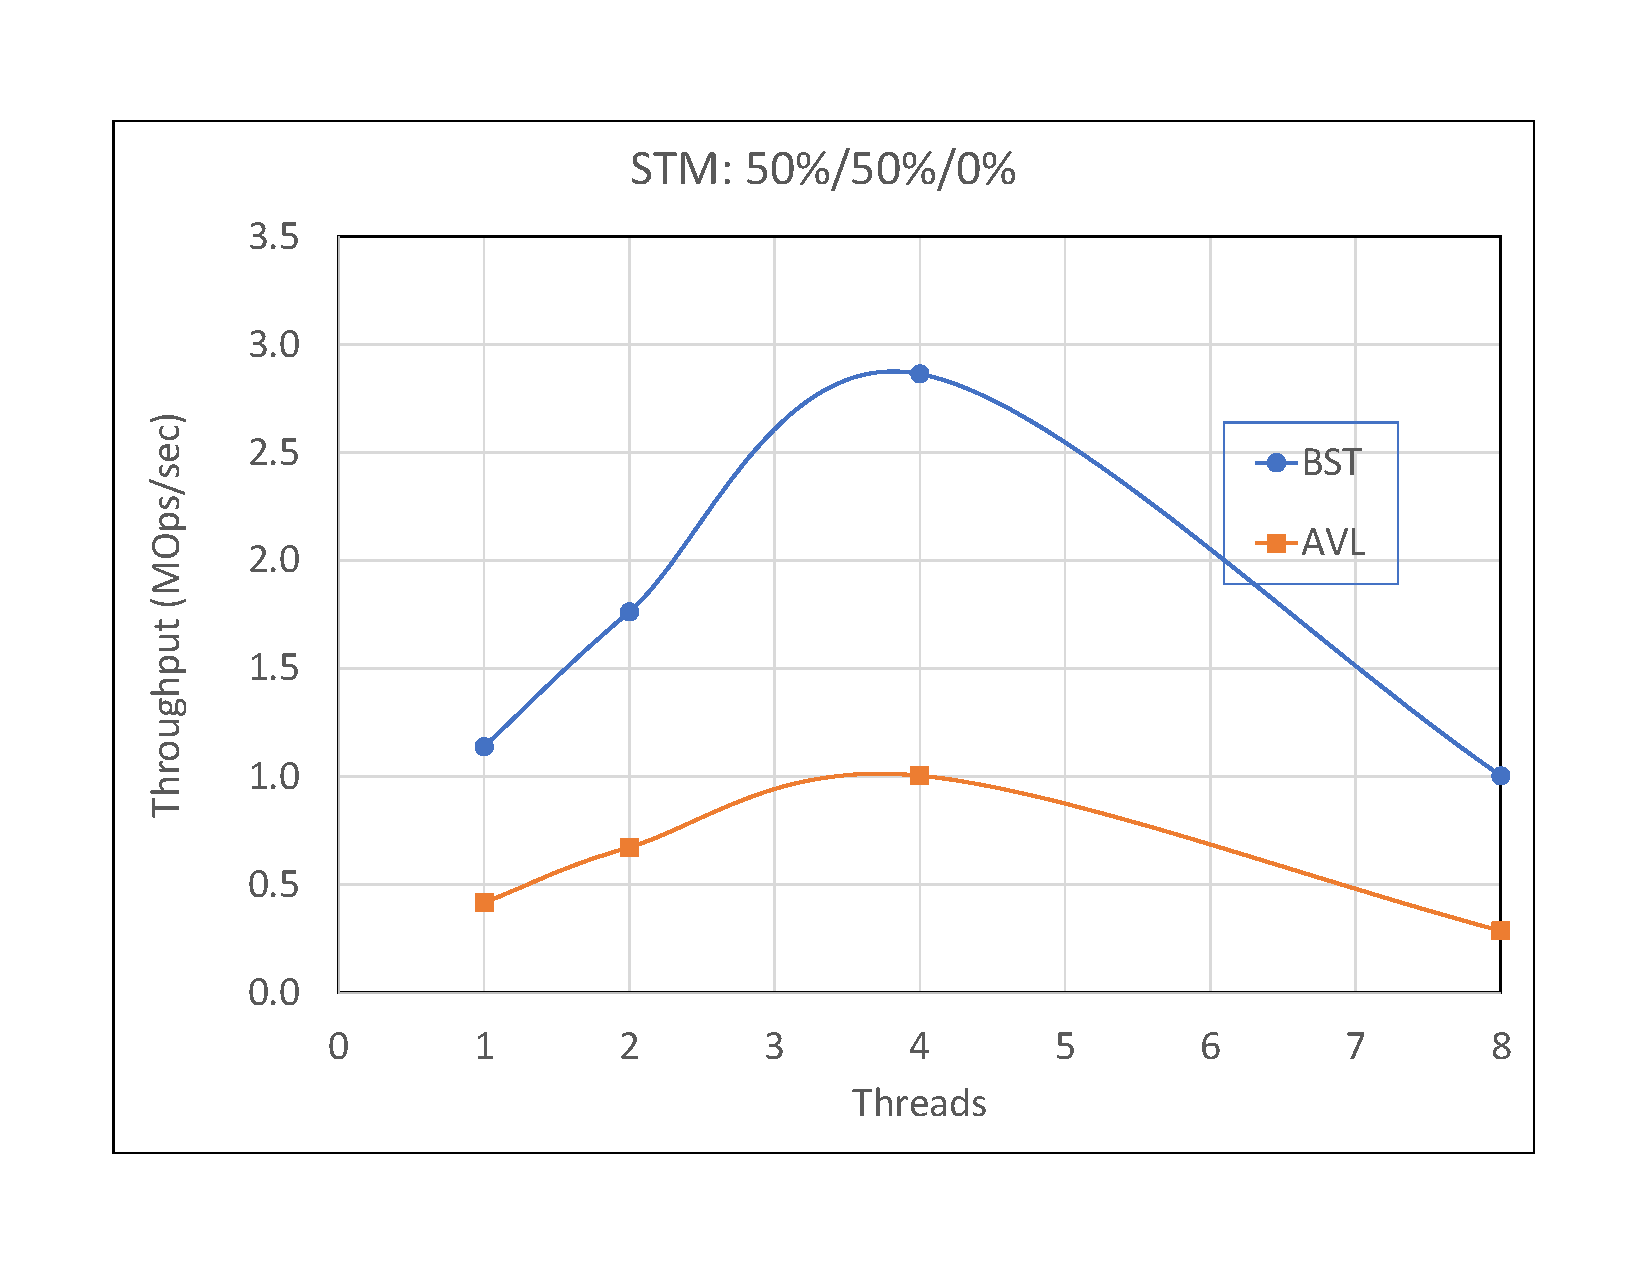
\includegraphics[width =\linewidth]{figures/stm1-50-50-0} \\
(c) 
\end{tabular}
\caption{adsf}
\end{figure}

\begin{figure}[H]
\begin{tabular}{c}
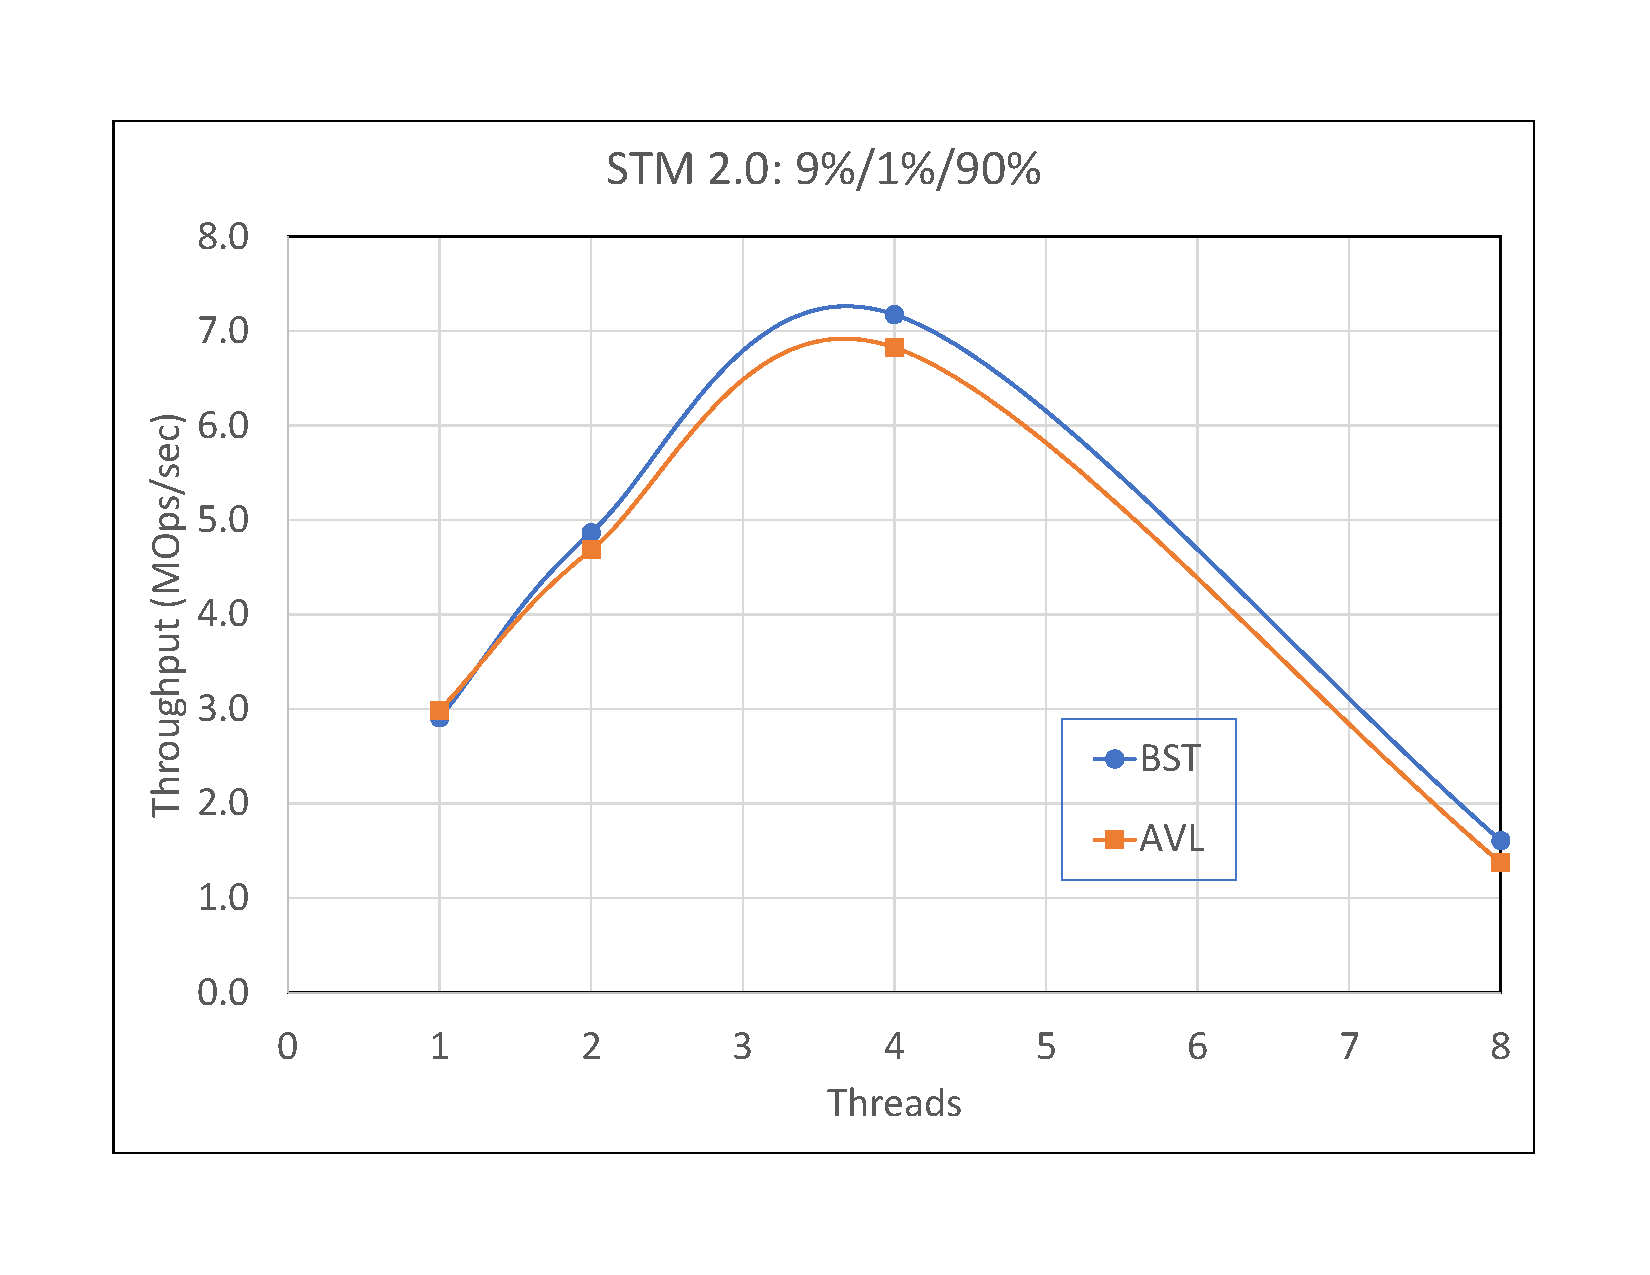
\includegraphics[width =\linewidth]{figures/stm2-9-1-90}\\
(a) \\
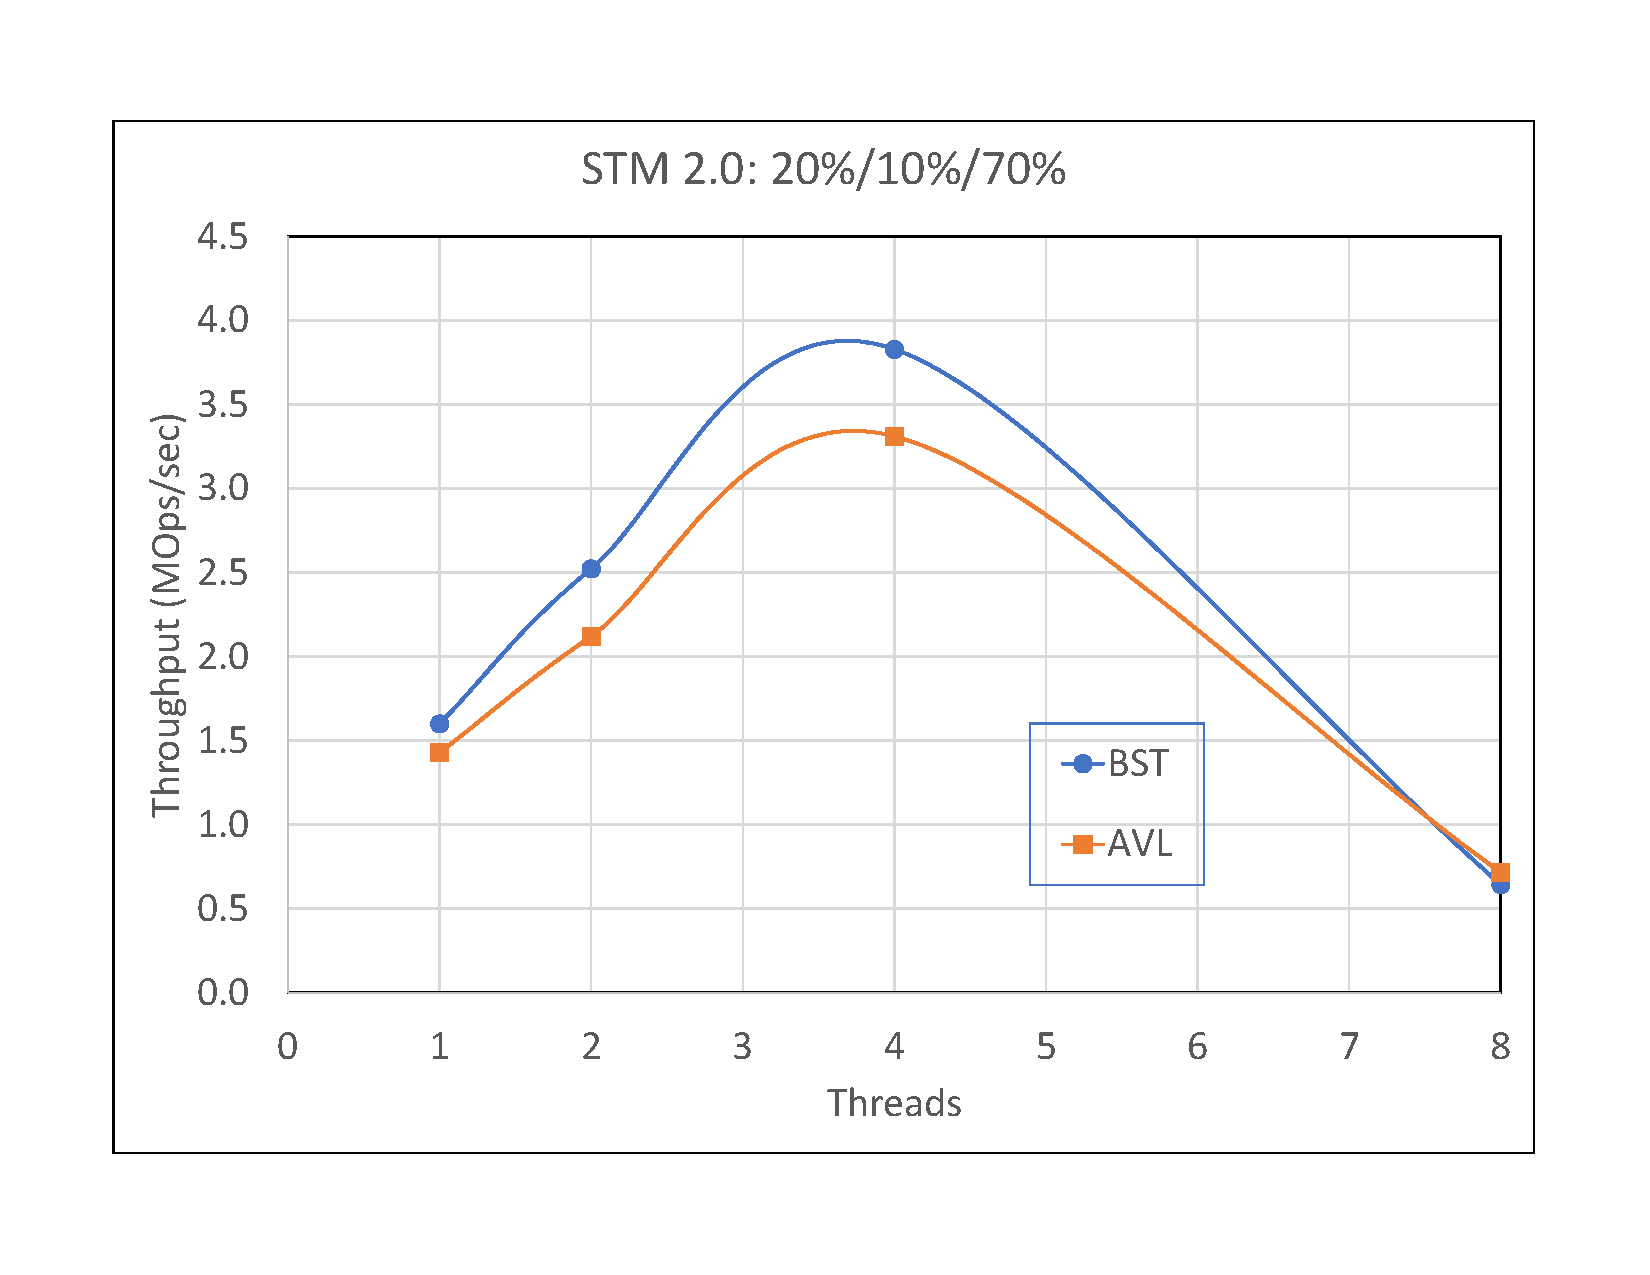
\includegraphics[width =\linewidth]{figures/stm2-20-10-70}\\
(b) \\
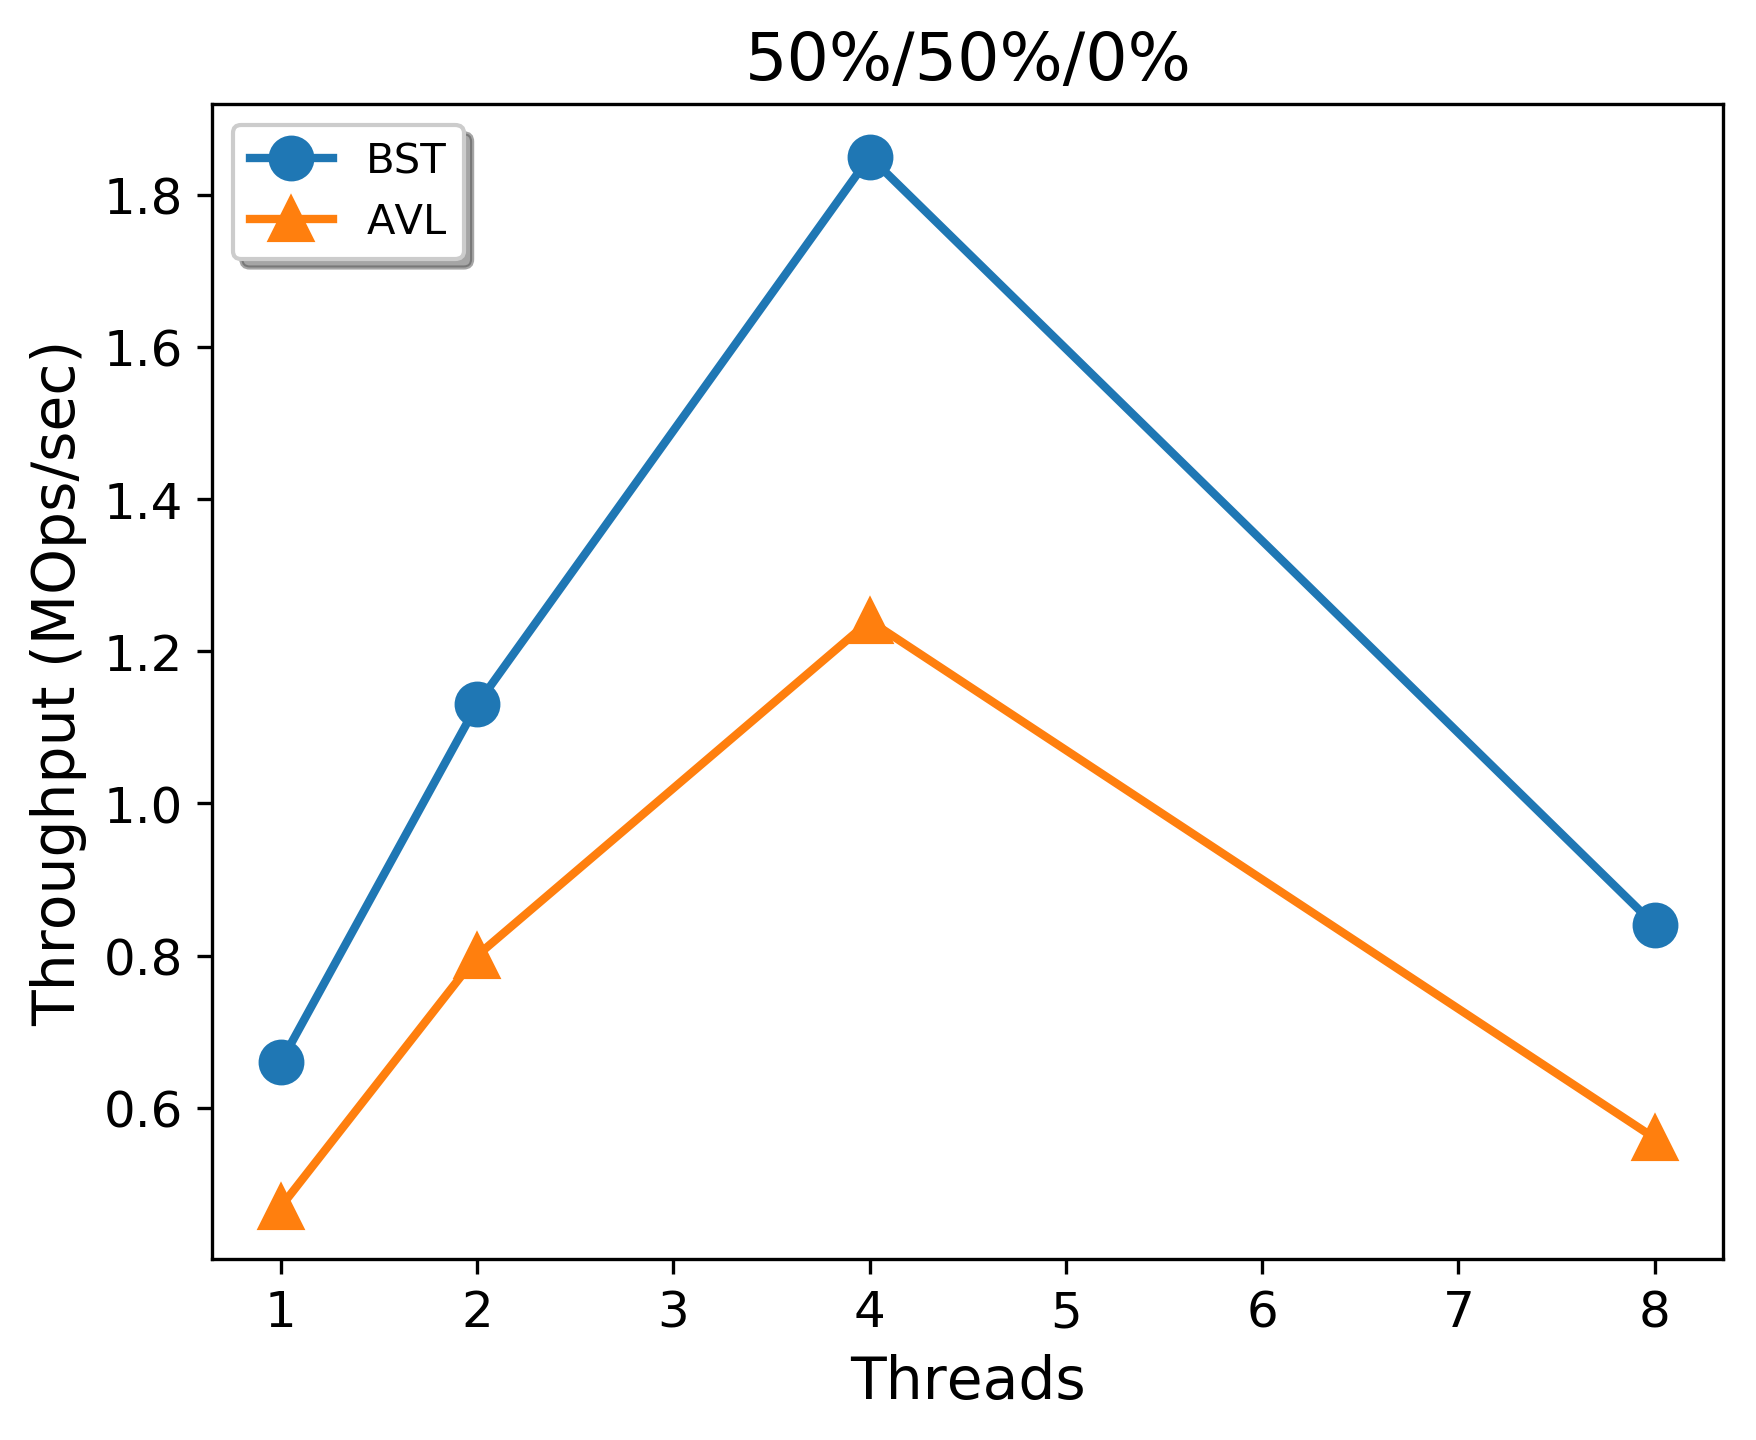
\includegraphics[width =\linewidth]{figures/stm2-50-50-0} \\
(c) 
\end{tabular}
\caption{adsf}
\end{figure}


\section{Appendix}

\section{Dictionary}
\begin{itemize}[label=$\ast$]
	\item Concurrency
	\item Logical ordering information
	\item Binary Search Tree
	\item AVL Tree
	\item Transactional Data Structure
	\item Software Transactional Memory
	\item Snapshots
	\item Succinct Path Snapshots
	\item HyperThreading
	\item Atomicity 
	\item Isolation
\end{itemize}

\section*{Acknowledgment}

\section*{References}

% TODO: FIX REFERENCES
%Practical Concurrent Traversals in Search Trees 
%http://webee.technion.ac.il/~idish/ftp/TransactionalLibrariesPLDI16.pdf - Transactional Data Structure Libraries
%http://webee.technion.ac.il/~idish/ftp/TransactionalLibrariesPLDI16.pdf



\begin{thebibliography}{00}
\bibitem{b1} Dana Drachsler-Cohen, Martin Vechev, and Eran Yahav. 2018. Practical concurrent traversals in search trees. In Proceedings of the 23rd ACM SIGPLAN Symposium on Principles and Practice of Parallel Programming (PPoPP '18). ACM, New York, NY, USA, 207-218. DOI: https://doi.org/10.1145/3178487.3178503
\bibitem{b2} Dana Drachsler-Cohen, Martin Vechev, and Eran Yahav. 2014. Practical Conccurent Binary Search Trees via Logical Ordering. http://www.cs.technion.ac.il/~yahave/papers/ppopp14-trees.pdf
\bibitem{b3} Dana Drachsler-Cohen, Martin Vechev, and Eran Yahav. 2014. Practical Conccurent Binary Search Trees via Logical Ordering. https://pdfs.semanticscholar.org/f776/1f31061936218458163adaa019f6f59a9030.pdf (Slides)

\end{thebibliography}

\end{document}
